% !TeX root = ../../pythonTutorial.tex
\label{machineLeaerning}

\section{Maschinelles Lernen in Python}\label{maschinelleslernen:einleitung}
Das Themengebiet des maschinellen Lernens kann verschiedene Komplexit�tslevel erreichen. Grundlegend ist das mathematische Verst�ndnis �ber die verschiedenen im maschinellen lernen eingesetzten Algorithmen. Diese werden in diesem Tutorial nicht beschrieben. \\
Sind die Algorithmen bekannt und sollen nun mittels Python angewendet werden, sollte zu Beginn mit einem kleinen Projekt gestartet werden. Hierbei ist es sinnvoll sich bereits am Anfang eine Vorgehensweise zu �berlegen, wie auch bei allen anderen Projekten. Python bietet im Bereich des maschinellen Lernens viele unterschiedliche M�glichkeiten an, sodass bereits fr�hzeitig der Aufbau des Projekts entschieden werden sollte. Grob kann ein Projekt in f�nf Schritte aufgeteilt werden, anhand derer sp�ter das Ergebnis verifiziert werden kann. \\

\begin{enumerate}
\item zu l�sendes Problem definieren
\item Daten verstehen und vorbereiten
\item m�gliche Algorithmen evaluieren
\item Ergebnisse verbessern
\item Ergebnisse darstellen
\end{enumerate}


Eine weit verbreitete M�glichkeit ist das Einbinden von bereits existierenden Bibliotheken, die viele Funktionalit�ten von Haus aus anbieten. Eine eigene Nachbildung von verbreiteten Algorithmen aus dem Bereich Maschinelles Lernen ist daher meist nicht n�tig.\\
Eine zweite M�glichkeit ist die Integration von R. Bei R handelt es sich um eine eigene Programmiersprache, welche den Schwerpunkt in mathematischen Probleml�sungen hat. Python und R lassen sich beide sowohl eigenst�ndig, also auch in Verbindung miteinander einsetzen.

Im Folgenden Abschnitt gibt es eine �bersicht, �ber wichtige und bekannte Bibliotheken aus dem Bereich maschinelles Lernen. Die Anzahl der Bibliotheken macht den Einstieg nicht ganz leicht. Die St�rken und Schw�chen der einzelnen Bibliotheken sollten betrachtet werden.

\subsection{Bibliotheken}\label{maschinelleslernen:bibliotheken}
Im Bereich maschinelles Lernen sind schon viele Bibliotheken vorhanden, die unterschiedliche Schwerpunkte in dem Bereich bedienen. Aus diesem Grund erfolgt zuerst eine �bersicht �ber verbreitete Bibliotheken.

Alle Bibliotheken\randnotiz{Download und Installation} die genutzt werden sollen m�ssen zuerst installiert werden. Hierf�r gibt es je nach Bibliothek und teilweise je nach Betriebssystem mehrere Wege. Es wird empfohlen hier aus der jeweiligen Webseite die geeignetsten Variante zu w�hlen und auszuf�hren.

Nach der Installation\randnotiz{Versionen und Kompatibilit�t} sollten alle Versionen ausgelesen und abgeglichen werden. Die Kompatibilit�t ist nicht durchgehend gew�hrleistet, das betrifft vor allem die unterschiedlichen Python-Versionen.

Der folgende Codeausschnitt zeigt ein Beispiel. Dieser kann entweder direkt in der Eingabeaufforderung bzw. Konsole nach Start von Python ausgef�hrt werden oder innerhalb einer geeigneten Entwicklungsumgebung.

\begin{lstlisting}
# Python version
import sys
print("Pyton: {}".format(sys.version))

# numpy version
import numpy
print("numpy: {}".format(numpy.__version__))

# pandas version
import pandas
print("pandas: {}".format(pandas.__version__))

# rpy2 version
import rpy2
print("rpy2: {}".format(rpy2.__version__))
\end{lstlisting}\label{maschinelleslernen:lst:printversions}

Die Ausgabe ist beispielsweise die Folgende:
\begin{lstlisting}
Pyton: 3.6.1 (v3.6.1:69c0db5, Mar 21 2017, 17:54:52) 
	[MSC v.1900 32 bit (Intel)]

numpy: 1.13.3 
pandas: 0.21.0
rpy2: 2.8.6
\end{lstlisting}\label{maschinelleslernen:lst:versions}

Auf diese Art und Weise sollten alle Bibliotheken gepr�ft werden, da so eventuelle Kompatibilit�tsprobleme oder fehlerhafte Installation fr�hzeitig erkannt werden k�nnen.

\subsubsection{Bekannte Bibliotheken}\label{maschinelleslernen:bekanntebibliotheken}
Grob kann man zwischen Datenanalyse und Visualisierung unterscheiden. Zwei bekannte Bibliotheken aus dem Bereich Datenanalyse sind \lstinline$numpy$ und \lstinline$pandas$, mit denen beispielsweise Gleichungen und Optimierungsprobleme gel�st werden k�nnen. Ergebnisse solcher Berechnungen k�nnen beispielsweise mithilfe des Moduls \lstinline$matplotlib$ visualisiert werden.~\cite{Python3}



In der Bibliothek \lstinline$numpy$~\cite{numpyreference} \randnotiz{Bibliothek numpy} wird ein flexibler Datentyp f�r mehrdimensionale Arrays zur Verf�gung gestellt. Dies erm�glicht eine effiziente Durchf�hrung von komplexen Rechnungen.

Au�erdem lassen sich Integrale berechnen, statistische Berechnungen durchf�hren und auch simulieren. All das wird f�r maschinelles Lernen ben�tigt. Da die Berechnungen mit Routinen nah an der Hardware durchgef�hrt werden, lassen sich bei entsprechender Programmierung effiziente Programme schreiben.

Die Arrays in \lstinline$numpy$ sind dreidimensional und k�nnen so eine Vielzahl von Anwendungsf�llen abbilden. Der Fokus von \lstinline$numpy$ liegt in der Datenhaltung und Manipulation von Daten. Hier speziell die numerische Manipulation aus dem Bereich der linearen Algebra. Mit den Matrizen k�nnen beispielsweise Multiplikationen und Dekompositionen durchgef�hrt werden. Aus diesem Grund sind \lstinline$numpy$-Array oft die Datenstruktur, mit der weiterf�hrende Bibliotheken arbeiten k�nnen.



Die Webseite zu \lstinline$pandas$~\cite{pandas} \randnotiz{Bibliothek pandas} beschreibt dieses als gute Wahl zur schnellen und flexiblen Aufbereitung von Daten. \lstinline$pandas$ bietet verschiedene M�glichkeiten, um schnell auf Eintr�ge zuzugreifen. Dies ist m�glich, da mittels \lstinline$pandas$ Serien und Dataframes erzeugt werden k�nnen, die im Gegensatz zu einem Array in Python auch Spaltentitel und Indizes anbieten.

Die \lstinline$describe()$-Methode bietet hierbei einen ersten �berblick �ber die im Dataframe enthalten Daten. Ohne weitere Programmierung werden Informationen wie Maximalwert, Minimalwert und Durchschnitt f�r jede Spalte berechnet und angezeigt. 

Spalten und Zeilen k�nnen mittels \lstinline$pandas$ gefiltert, erweitert und ver�ndert werden, sodass \lstinline$pandas$ oft im ersten Schritt genutzt wird, um die auszuwertenden Daten zu laden und genauer analysieren zu k�nnen.


Erg�nzend bzw. aufbauen auf \lstinline$numpy$ \randnotiz{Bibliothek scipy} werden durch \textit{scipy}~\cite{scipyreference} viele mathematische Operationen bereit gestellt. 
Das Modul \lstinline$scipy$ ist sehr m�chtig und daher nochmal in Untermodule aufgeteilt. Innerhalb der Untermodule werden bestimmte Funktionalit�ten gruppiert. Eine �bersicht hierzu gibt die Onlinedokumentation.



Viele DataMining \randnotiz{Bibliothek scikit-learn} bzw. Machine Learning Funktionalit�ten werden bereits durch die \textit{scikit-learn}~\cite{scikit} Bibliothek (manchmal aus sklearn abgek�rzt) zur Verf�gung gestellt. Die klassischen Algorithmen, wie \lstinline$k-Means$ oder \lstinline$knn$ sind bereits integriert.\\
Des Weiteren ist auch mit \lstinline$scikit-learn$ eine Aufbereitung der Daten m�glich. Hier werden beispielsweise Normalisierung und Skalierung unterst�tzt. Insgesamt handelt es sich um eine sehr m�chtige Bibliothek, mit der es m�glich ist unterschiedliche Algorithmen zu probieren und verschiedene Test- und Trainingsverfahren zu testen. Es k�nnen auch neue Daten anhand der gelernten Modelle klassifiziert und vorhergesagt werden.



Eine weitere M�glichkeit\randnotiz{Bibliothek rpy2} ist das Einbinden des Pakets \lstinline$rpy2$~\cite{rpy2}. Hierbei handelt es sich um eine Bibliothek, welche Komponenten aus R zur Verf�gung stellt. \lstinline$rpy2$ ist zu sehen wie eine Schnittstelle zwischen Python und R. Es ist m�glich R-Pakete mittels Python zu importieren und mit den darin enthaltenen Funktionalit�ten zu interagieren.



Mit dem Modul \lstinline$matplotlib$~\cite{matplotlib} \randnotiz{Bibliothek matplotlib} k�nnen Daten in einem Diagramm dargestellt werden. Hiermit kann ein erstes Verst�ndnis der Daten oder Ergebnisse erreicht werden. Es werden unter anderem Liniendiagramme, Histogramme, Balkendiagramme aber auch Heatmaps unterst�tzt. Hier k�nnen sowohl Achsen, Farben und auch Beschriftungen nach Bedarf angepasst werden. \lstinline$matplotlib$ unterst�tzt sowohl \lstinline$pandas$ als auch \lstinline$numpy$ und ist daher oft bereits am Anfang von hoher Bedeutung, um einen �berblick �ber die Daten zu bekommen.

\uebung
\aufgabe{MachineLearning/machinelearning_questions}

\uebung
\aufgabe{MachineLearning/machinelearning_questions}

\subsection{Einfache Anwendungsbeispiele}\label{maschinelleslernen:anwendungsbeispiele}
Es gibt verschiedene Herangehensweisen, meist bietet es sich an, erst mal einen groben �berblick �ber die Daten zu erhalten. F�r die erste Erl�uterung werden Datens�tze angenommen, welche in folgender Datenstruktur vorliegen.

\subsubsection*{Daten aus Datei lesen und anzeigen}
Maschinelles Lernen \randnotiz{Beispieldaten} macht nur Sinn mit entsprechenden Daten. Diese sollten im Besten Fall bereits in einer strukturierten Form vorliegen.
\lstinputlisting[language=Python]{chapters/advancedTopics/src/machinelearning/datasample1.txt}\label{datasample1:lst:datasample}


Nun kann mit der Entwicklung begonnen werden. Um den Datentyp \randnotiz{Datei lesen} mit Daten zu versorgen findet sich im Folgenden ein kleiner Codeausschnitt:
\lstinputlisting{chapters/advancedTopics/src/machinelearning/readdatafromfile.py}\label{readdatafromfile:lst:readdata}

Die aufbereiteten Daten k�nnen im n�chsten Schritt visualisiert werden. Vorher noch eine weitere Variante wie Daten geladen werden k�nnen.

\subsubsection*{Daten aus Paket laden}
Eine\randnotiz{iris-Dataset laden} weitere M�glichkeit ist das Laden von Daten aus Paketen. Hier wird beispielhaft das Lesen aus dem Paket \lstinline$iris$ vorgestellt.
\lstinputlisting[language=Python,firstline=3,lastline=19]{chapters/advancedTopics/src/machinelearning/loadiris.py}\label{loadiris:lst:loadiris}

Nun kann es an die Darstellung der Daten gehen.

\subsubsection*{Plots erzeugen}
Aus den oben gelesen Daten kann nun ein Plot erzeugt werden. F�r das Beispiel oben bietet sich die Darstellung in einem Scatterplot an.


\randnotiz{Plot erzeugen}\lstinputlisting[language=Python]{chapters/advancedTopics/src/machinelearning/defineplot1.py}\label{defineplot1:lst:2dplot}

Eine Darstellung in 3D ist ebenfalls m�glich. Hierzu wird aus dem DataSet noch eine dritte Dimension ausgelesen.

\randnotiz{3 Achsen}\lstinputlisting[language=Python]{chapters/advancedTopics/src/machinelearning/defineplot2.py}\label{defineplot2:lst:3dplot}


\uebung
\aufgabe{MachineLearning/machinelearning_simple}

\subsection{Beispiel: knn-Klassifikation}\label{maschinelleslernen:knnklassifikation}
Der knn-Algorithmus ist einer der bekanntesten Algorithmus aus dem Bereich Klassifikation und wird daher hier als Codebeispiel dargestellt und erl�utert.

Folgende Imports\randnotiz{Imports} sind f�r dieses Beispiel n�tig:
\lstinputlisting[language=Python,firstline=4,lastline=11]{chapters/advancedTopics/src/machinelearning/knnsample.py}\label{knnsample:lst:knnsample4}

Anschlie�end k�nnen die Daten\randnotiz{Daten laden} geladen und die Spaltennamen definiert werden.
\lstinputlisting[language=Python,firstline=14,lastline=20]{chapters/advancedTopics/src/machinelearning/knnsample.py}\label{knnsample:lst:knnsample14}

Jetzt werden die Daten gelesen\randnotiz{Daten lesen und vorbereiten} und vorbereitet.
\lstinputlisting[language=Python,firstline=22,lastline=28]{chapters/advancedTopics/src/machinelearning/knnsample.py}\label{knnsample:lst:knnsample22}

Zur Berechnung m�ssen die Daten\randnotiz{Daten skalieren} skaliert werden.
\lstinputlisting[language=Python,firstline=33,lastline=37]{chapters/advancedTopics/src/machinelearning/knnsample.py}\label{knnsample:lst:knnsample33}

Nun kann der KNN-Algorithmus\randnotiz{Algorithmus anwenden} angewendet werden.
\lstinputlisting[language=Python,firstline=39,lastline=44]{chapters/advancedTopics/src/machinelearning/knnsample.py}\label{knnsample:lst:knnsample39}

Jetzt k�nnen wir die Daten-Matrix\randnotiz{Matrix ausgeben} ausgeben.
\lstinputlisting[language=Python,firstline=46,lastline=47]{chapters/advancedTopics/src/machinelearning/knnsample.py}\label{knnsample:lst:knnsample46}

Als Ausgabe wird Folgendes angezeigt
\begin{lstlisting}
[[ 9  0  0]
 [ 0 12  1]
 [ 0  1  7]]
\end{lstlisting} 
 
Zus�tzlich\randnotiz{Report ausgeben} kann ein Report angezeigt werden, welcher eine gute �bersicht �ber die klassifizierten Daten gibt.
\lstinputlisting[language=Python,firstline=48,lastline=49]{chapters/advancedTopics/src/machinelearning/knnsample.py}\label{knnsample:lst:knnsample49}

Die Ausgabe ist die folgende:
\begin{lstlisting} 
                  precision    recall  f1-score   support
 
     Iris-setosa       1.00      1.00      1.00         9
 Iris-versicolor       0.92      0.92      0.92        13
  Iris-virginica       0.88      0.88      0.88         8
 
       micro avg       0.93      0.93      0.93        30
       macro avg       0.93      0.93      0.93        30
    weighted avg       0.93      0.93      0.93        30
\end{lstlisting}



Um \randnotiz{Fehler ausgeben}ein abschlie�endes Bild �ber die Klassifikation zu erhalten k�nnen nun noch die Fehler ausgegeben werden.
\lstinputlisting[language=Python,firstline=51,lastline=61]{chapters/advancedTopics/src/machinelearning/knnsample.py}\label{knnsample:lst:knnsample51}


Aus\randnotiz{Fehler-Plot erzeugen} den berechneten Fehlern bei der Klassifikation kann nun noch ein Plot erzeugt werden.
\lstinputlisting[language=Python,firstline=64,lastline=72]{chapters/advancedTopics/src/machinelearning/knnsample.py}\label{knnsample:lst:knnsample64}

Der Plot zeigt sich wie in Abbildung ~\ref{ml:samples:plotknn}.

\begin{figure}[ht]
	\centering
	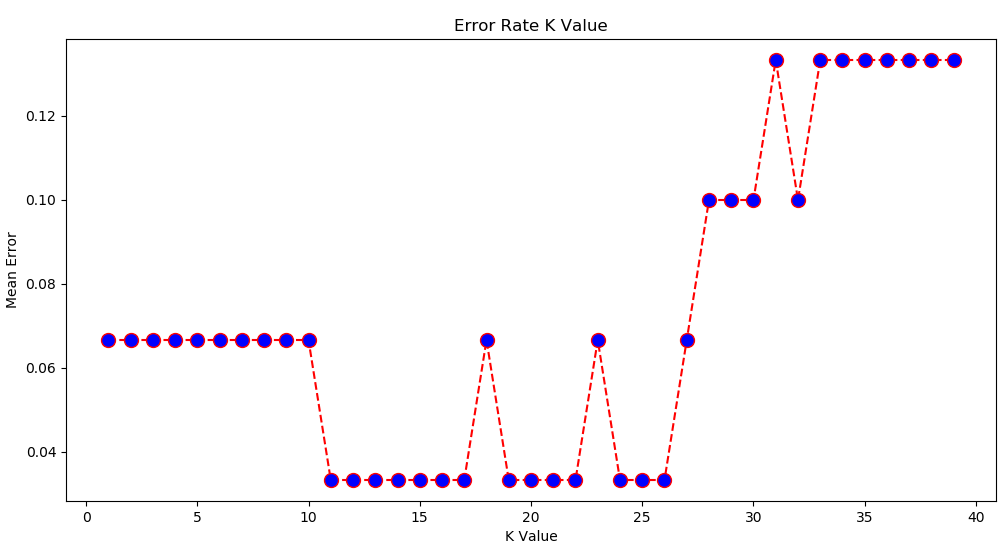
\includegraphics[width=1\textwidth]{images/MachineLearning/ml_knn_plot.png}
	\caption{Ergebnis-Plot der Fehler nach Ausf�hrung KNN}
	\label{ml:samples:plotknn}
\end{figure}

\uebung
\aufgabe{MachineLearning/machinelearning_knn}


\uebung
\aufgabe{MachineLearning/machinelearning_knn}

\subsection{Naive Bayes}\label{maschinelleslernen:naivebayes}
Ein weiteres Beispiel aus dem Bereich Klassifikation im maschinellen Lernen ist der Naive Bayes Algorithmus.

Es \randnotiz{Importe}sind wieder einige Importe n�tig.
\lstinputlisting[language=Python,firstline=3,lastline=5]{chapters/advancedTopics/src/machinelearning/bayessample.py}\label{knnsample:lst:bayessample3}

Die \randnotiz{Daten laden}Beispieldaten m�ssen definiert werden.
\lstinputlisting[language=Python,firstline=7,lastline=11]{chapters/advancedTopics/src/machinelearning/bayessample.py}\label{knnsample:lst:bayessample7}

Nun kann das Modell erzeugt werden um mit den Daten zu trainieren. Anschlie�end k�nnen die Daten vorhergesagt und die Ergebnisse anzeigt werden.
\lstinputlisting[language=Python,firstline=13,lastline=21]{chapters/advancedTopics/src/machinelearning/bayessample.py}\label{knnsample:lst:bayessample13}

Die Ausgabe lautet:
\begin{lstlisting}
[3 4]
\end{lstlisting}

\uebung
\aufgabe{MachineLearning/machinelearning_bayes}

\subsection{Beispiel: Lineare Regression}\label{maschinelleslernen:linregress}
Beispiel aus dem Bereich Regression. Konkret wird hier eine lineare Regression dargestellt. 

Es \randnotiz{Importe}sind verschiedene Importe f�r n�tig. Die werden im ersten Schritt importiert.
\lstinputlisting[language=Python,firstline=1,lastline=5]{chapters/advancedTopics/src/machinelearning/linregress.py}\label{knnsample:lst:lingress1}

Daten \randnotiz{Daten laden}aus boston-Datensatz auslesen und in numpy-array �berf�hren.
\lstinputlisting[language=Python,firstline=7,lastline=10]{chapters/advancedTopics/src/machinelearning/linregress.py}\label{knnsample:lst:lingress7}

Die \randnotiz{Berechnung durchf�hren}Berechnung der linearen Regression kann direkt aus dem scipy-Paket erfolgen. Die n�tigen Daten m�ssen mitgegeben werden.
\lstinputlisting[language=Python,firstline=12,lastline=13]{chapters/advancedTopics/src/machinelearning/linregress.py}\label{knnsample:lst:lingress12}

Nun \randnotiz{Plot erzeugen}kann der Plot f�r die berechneten Werte erzeugt werden.
\lstinputlisting[language=Python,firstline=15,lastline=27]{chapters/advancedTopics/src/machinelearning/linregress.py}\label{knnsample:lst:lingress15}


\begin{figure}[ht]
	\centering
	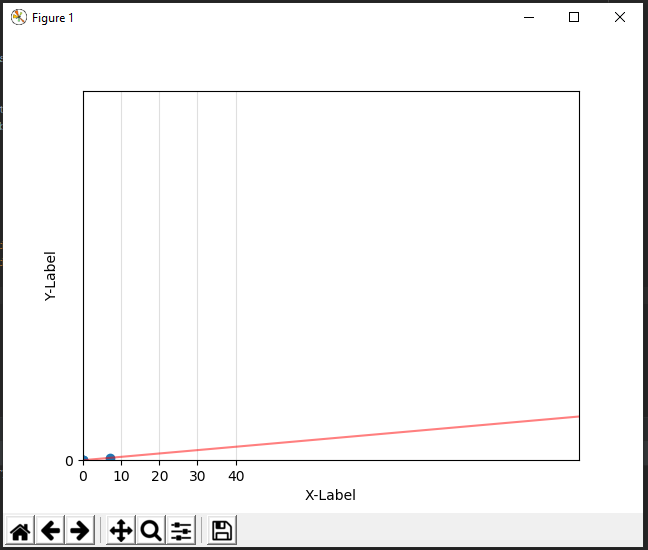
\includegraphics[width=0.9\textwidth]{images/PlotLinRegress.png}
	\caption{Ergebnis-Plot der linearen Regression}
	\label{ml:samples:plotlinregress}
\end{figure}

Somit haben wir nun auch eine lineare Regression erfolgreich durchgef�hrt.


\uebung
\aufgabe{MachineLearning/machinelearning_linregress}

\uebung
\aufgabe{MachineLearning/machinelearning_linregress}